\begin{frame}[fragile]{Receipt (execution output)}
  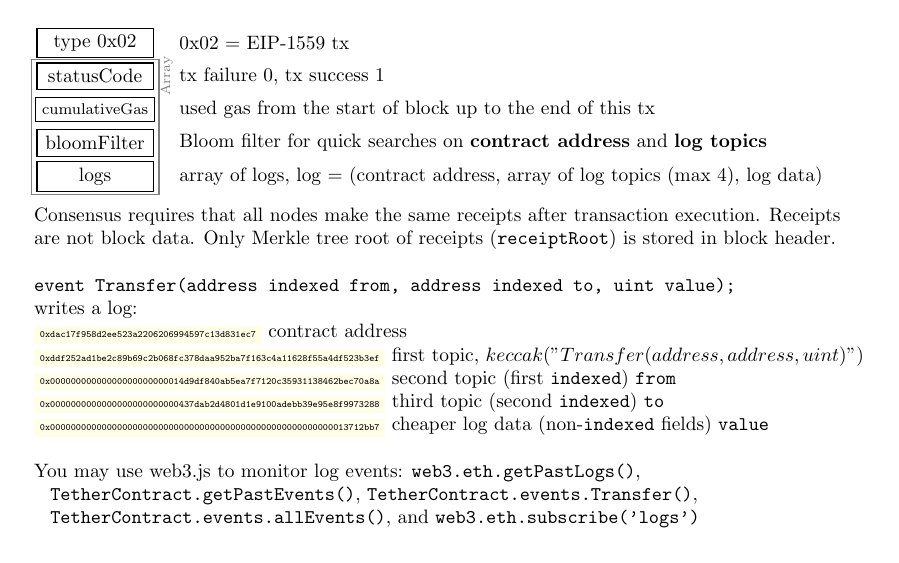
\begin{tikzpicture}[scale=0.7,every node/.style={transform shape}]
    \tikzstyle{field}=[minimum width=6em,minimum height=2.8ex,draw]
    \tikzstyle{desc}=[right=+4em]
    \node[field] at (0,0) {type 0x02};
      \node[desc] at (0,0) {0x02 = EIP-1559 tx};
    \node[field] at (0,-4ex) {statusCode};
      \node[desc] at (0,-4ex) {tx failure 0, tx success 1};
    \node[field] at (0,-8ex) {{\footnotesize cumulativeGas}};
      \node[desc] at (0,-8ex) {used gas from the start of block up to the end of this tx};
    \node[field] at (0,-12ex) {bloomFilter};
      \node[desc] at (0,-12ex) {Bloom filter for quick searches on \textbf{contract address} and \textbf{log topics}};
    \node[field] at (0,-16ex) {logs};
      \node[desc] at (0,-16ex) {array of logs, log = (contract address, array of log topics (max 4), log data)};

    \draw[gray] (-3.3em,-2ex) rectangle (3.3em,-18.2ex);
    \node[rotate=90,gray] at (3.7em, -4ex) {{\scriptsize Array}};

\node[align=left,anchor=north west] at (-3.5em,-19ex) {
Consensus requires that all nodes make the same receipts after transaction execution. Receipts\\
are not block data. Only Merkle tree root of receipts (\texttt{receiptRoot}) is stored in block header.\\
\\
\texttt{event Transfer(address indexed from, address indexed to, uint value);}\\
writes a log:\\
\texttt{\tiny \colorbox{yellow!10}{0xdac17f958d2ee523a2206206994597c13d831ec7}} contract address\\
\texttt{\tiny \colorbox{yellow!10}{0xddf252ad1be2c89b69c2b068fc378daa952ba7f163c4a11628f55a4df523b3ef}} first topic, $keccak("Transfer(address,address,uint)")$\\
\texttt{\tiny \colorbox{yellow!10}{0x00000000000000000000000014d9df840ab5ea7f7120c35931138462bec70a8a}} second topic (first \texttt{indexed}) \texttt{from}\\
\texttt{\tiny \colorbox{yellow!10}{0x0000000000000000000000000437dab2d4801d1e9100adebb39e95e8f9973288}} third topic (second \texttt{indexed}) \texttt{to}\\
\texttt{\tiny \colorbox{yellow!10}{0x0000000000000000000000000000000000000000000000000000000013712bb7}} cheaper log data (non-\texttt{indexed} fields) \texttt{value}\\
\\
You may use web3.js to monitor log events: \texttt{web3.eth.getPastLogs()},\\
\hspace{0.5em} \texttt{TetherContract.getPastEvents()}, \texttt{TetherContract.events.Transfer()},\\
\hspace{0.5em} \texttt{TetherContract.events.allEvents()}, and \texttt{web3.eth.subscribe('logs')}
};

  \end{tikzpicture}
\end{frame}